\documentclass[border=0.2cm]{standalone}
\usepackage{tikz}
\usetikzlibrary{intersections,calc}
\begin{document}


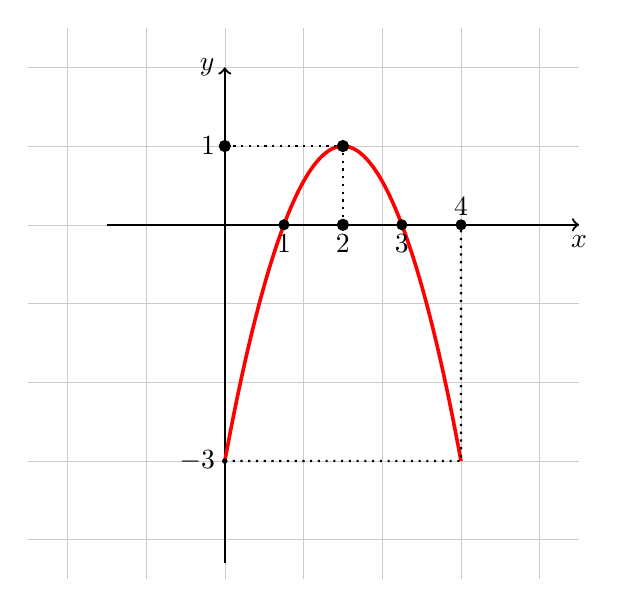
\begin{tikzpicture}

  \coordinate (a) at (-1.5,-3);
  \coordinate (by) at ($(a) + (1.5,4)$);  %($(b) + (-1.5,-1)$)
  \coordinate (bx) at ($(a) + (0,5)$);  %($(b) + (-1.5,-1)$)
  \coordinate (b) at ($(a) + (1.5,5)$);  %($(b) + (-1.5,-1)$)

  \draw[help lines,black!20,xshift=-15mm] (-2.5,-3.5) grid (4.5,3.5);
  \draw[thick,->,name path=xline] (-3,1) -- (3,1) node[below] {$x$};
  \draw[thick,->] (-1.5,-3.3) -- (-1.5,3)   node[left]  {$y$};
  \draw[line width=1.3pt,red,name path=parabola] (-1.5,-2) parabola bend (0,2) (1.5,-2);
  \fill (-1.5,-2) circle (1pt) node[left] {$-3$};
  \fill (bx) circle (1pt) node[left] {$1$};
  \draw[fill] (b)  circle (2pt); %node[left] {(b)};
  \draw[fill] (by) circle (2pt); %node[left] {(by)};
  \draw[fill] (bx) circle (2pt); %node[left] {(bx)};
 
  \draw[thick, dotted] (by)node[below] {2} -- (b) -- (bx);
  \draw[thick, dotted] (-1.5,-2) -- +(3,0) -- (1.5,1);
  \fill (1.5,1) circle (2pt) node [above] {4};

  \fill[name intersections={of=xline and parabola}] (intersection-1) circle (2pt) node[below] {1}; 
  \fill[name intersections={of=xline and parabola}] (intersection-2) circle (2pt) node[below] {3};
  

\end{tikzpicture}
\end{document}